\section{From Perceptrons to Feed Forward Neural Networks}
Guardati le slides per la prima parte.

\subsection{A Note on Maximum Likelihood Estimation}
The goal of \textbf{Maximum Likelihood} estimation is to make inferences about the population that is most likely to have generated the sample.
Maximum likelihood estimation is a method of estimating the parameters of a probability distribution by maximizing a likelihood function, so that under the assumed statistical model the observed data is most probable. The main appeal of this method derives from the fact that it can be shown to be the best estimator asymptotically (as the number of examples $m \to \infty$) in terms of its rate of convergence as $m$ increases. Under appropriate conditions, as the number of samples goes to infinity, the maximum likelihood estimate of a parameter converges to the true value of a parameter; this property is called \textit{consistency}. 

Let's observe independent identically distributed samples from a Gaussian distribution with known $\sigma^2$:
\begin{center}
    $x_{1}, x_{2}, \ldots, x_{N} \sim N\left(\mu, \sigma^{2}\right) \quad p\left(x | \mu, \sigma^{2}\right)=\frac{1}{\sqrt{2 \pi} \sigma} e^{-\frac{(x-\mu)^{2}}{2 \sigma^{2}}}$  
\end{center}
Let $\theta = (\theta_1,...,\theta_p)^T$ a vector of parameters, we want to find the MLE for $\theta$; we do the following:
\begin{itemize}
    \item write the likelihood $L=P(Data|\theta)$ for the data;
    \item take the logarithm of the likelihood $l=logP(Data|\theta)$, which is called the \textbf{log-likelihood}; this has several advantages, for example for a numerical point of view the product is more prone to underflow;
    \item find the maximum solving $\frac{\partial l}{\partial\theta_i}=0$.
\end{itemize}
The likelihood of the data can be expressed as follows:
\begin{center}
    $L(\mu)=p\left(x_{1}, x_{2}, \ldots, x_{N} | \mu, \sigma^{2}\right)=\prod_{n=1}^{N} p\left(x_{n} | \mu, \sigma^{2}\right)$
$=\prod_{n=1}^{N} \frac{1}{\sqrt{2 \pi} \sigma} e^{\frac{\left(x_{n}-\mu\right)^{2}}{2 \sigma^{2}}}$   
\end{center}
We can transform the product in a sum by taking the logarithm, having the log-likelihood:
\begin{center}
    $\begin{aligned} l(\mu)=\log \left(\prod_{n=1}^{N} \frac{1}{\sqrt{2 \cdot \pi} \sigma} e^{-\frac{\left(x_{n}-\mu\right)^{2}}{2 \cdot \sigma^{2}}}\right)=& \sum_{n=1}^{N} \log \frac{1}{\sqrt{2 \cdot \pi} \sigma} e^{-\frac{\left(x_{n}-\mu\right)^{2}}{2 \cdot \sigma^{2}}}=\\ &=N \cdot \log \frac{1}{\sqrt{2 \cdot \pi} \sigma}-\frac{1}{2 \cdot \sigma^{2}} \sum_{n}^{N}\left(x_{n}-\mu\right)^{2} \end{aligned}$   
\end{center}
Find out the derivative, noting that the first part does not depend on $\mu$:
\begin{center}
    $\frac{\partial l(\mu)}{\partial \mu}=\frac{\partial}{\partial \mu}\left(N \cdot \log \frac{1}{\sqrt{2 \pi} \sigma}-\frac{1}{2 \sigma^{2}} \sum_{n}^{N}\left(x_{n}-\mu\right)^{2}\right)=$
$=-\frac{1}{2 \sigma^{2}} \frac{\partial}{\partial \mu} \sum_{n}^{N}\left(x_{n}-\mu\right)^{2}=-\frac{1}{2 \sigma^{2}} \sum_{n}^{N} 2\left(x_{n}-\mu\right)$
\end{center}
Solve the set of simultaneous equations $\frac{\partial l}{\partial\theta_i}=0$:
\begin{center}
    $-\frac{1}{2 \sigma^{2}} \sum_{n}^{N} 2\left(x_{n}-\mu\right)=0$ \\ $\sum_{n}^{N}\left(x_{n}-\mu\right)=0$ \\
    $\sum_{n}^{N} x_{n}=\sum_{n}^{N} \mu $ \\
    \vspace{0.5cm}
    $\mu^{M L E}=\frac{1}{N} \sum_{n}^{N} x_{n}$
\end{center}
As we can see, the $\mu^{MLE}$ is the average of the $x_n$, so the sample mean is an estimate of the mean and this comes from the fact that you are doing a maximum likelihood estimation of the mean of a Gaussian distribution. This is an unbiased estimator, so it's a nice estimator and we'd like to do the same with neural networks.

\subsection{Neural Networks for Regression}
You want to find the weights so that this network approximates some target value.
\begin{center}
    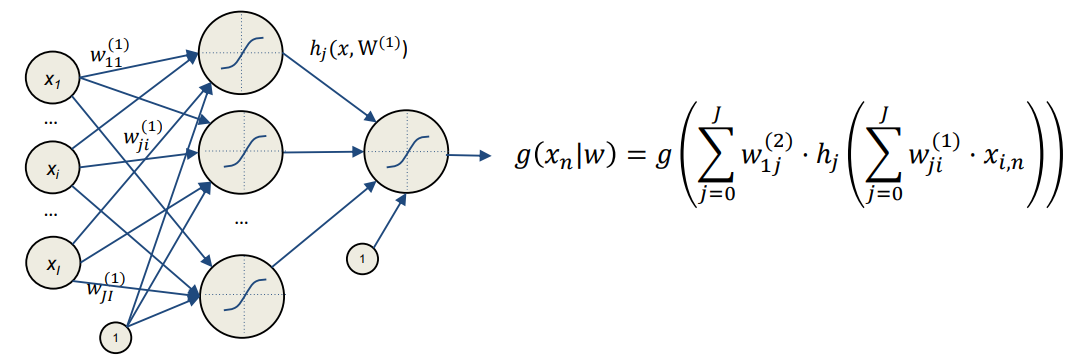
\includegraphics[width=0.8\textwidth]{images_1/per6.png}    
\end{center}
Let's assume $\textbf{t}$ as the function we want to approximate with $N$ observations.
\begin{center}
    $t_{n}=g\left(x_{n} | w\right)+\epsilon_{n}, \quad \epsilon_{n} \sim N\left(0, \sigma^{2}\right)$ 
\end{center}
Let's assume that this network is so good for some weights that besides some noise it is exactly equal to the function 
%(slide 41)
; so let's assume that this data really comes from this network but has been corrupted by noise. I assume that the difference between the prediction and the target is an error which comes from a Gaussian distribution with some noise; this is one possible assumption, we'll take this. We will approximate $t$ as:
\begin{center}
    $t_n \sim N(g(x_n|w),\sigma^2)$
\end{center}
So we have i.i.d samples coming from a Gaussian distribution as follows:
\begin{center}
    $t_n \sim N(g(x_n|w),\sigma^2)$
    
    $p(t|g(x|w),\sigma^2)=\frac{1}{\sqrt{2\pi}\sigma}e^{-\frac{(t-g(|w))^2}{2\sigma^2}}$
\end{center}
Let's try to compute the maximum likelihood %of the mean 
as a function of the weights, which are our parameters. The likelihood is the joint probability of all the observations [in case of a Gaussian distribution]: 
$$
L(w)=p(t_1, t_2, ..., t_N | g(x|w), \sigma^2)=\prod_{n=1}^{N} p\left(t_{n} |g\left(x_{n} | w\right), \sigma^{2}\right)=
\prod_{n=1}^{N} \frac{1}{\sqrt{2 \pi} \sigma} e^{-\frac{\left(t_{n}-g\left(x_{n} | w\right)\right)^{2}}{2 \sigma^{2}}}
$$
%we need to know the likelihood of the data which is for a Gaussian the joint probability of all the observations, which means the product of the observations:
Look for the weights which maximize the likelihood: 
\begin{center}
    $\operatorname{argmax}_{w} L(w)=\operatorname{argmax}_{w} \prod_{n=1}^{N} \frac{1}{\sqrt{2 \pi} \sigma} e^{-\frac{\left(t_{n}-g\left(x_{n} | w\right)\right)^{2}}{2 \sigma^{2}}}$
\end{center}
These are the canonic Gaussian but the mean is replaced with $g\left(x_{n} | w\right)$, which means a function parametrized in a given set of parameters $w$ evaluated in x. You want to compute the maximum of the likelihood; instead of product we can take the logarithm:
$$
\operatorname{argmax}_{w} \sum_{n}^{N} \log \left(\frac{1}{\sqrt{2 \pi} \sigma} e^{-\frac{\left(t_{n}-g\left(x_{n} | w\right)\right)^{2}}{2 \sigma^{2}}}\right)=\operatorname{argmax}_{n} \sum_{n}^{N} \log \frac{1}{\sqrt{2 \pi} \sigma}-\frac{1}{2 \sigma^{2}}\left(t_{n}-g\left(x_{n} | w\right)\right)^2
$$
We can see that $-\frac{1}{2 \sigma^{2}}$ is a negative constant so we have to remove it by changing the sign of this function: instead of maximize we have to minimize. The max likelihood weights are obtained by minimizing this:
\begin{center}
    $ \operatorname{argmin}_{w} \sum_{n}^{N}\left(t_{n}-g\left(x_{n} | w\right)\right)^{2} $
\end{center}
%So the keypoint of using the sum of squares errors is that you are assuming this; under this assumptions finding the weights that minimize the sum of squares errors means to estimate the weights with the max like approach. 
What if our error does not come from a Gaussian distribution? If the error is not a Gaussian distribution, you can still do this but it's not the best solution and it's not a maximum likelihood estimation so you might end up with a solution that is not unbiased (unbiased means an estimator with zero bias). 
But if you know that the errors are distributed differently you can follow the process and you will get the exact solution. 

\subsection{Neural Networks for Classification}
Let's start with a very well known problem: \textit{Classification}. Let's talk about binary classification: the output is either 0 or 1
%, so the output of the network can only be distributed as a distribution that outputs 0 or 1.
Let's assume our model now estimates the probability of class 1, instead of the class 0, for example using a sigmoid function. We can assume that the target comes from a Bernoulli distribution and the network is basically estimating what is the probability of 1 (or 0, equally). 
\begin{center}
    $g\left(x_{n} | w\right)=p\left(t_{n} | x_{n}\right), \quad t_{n} \in\{0,1\} \quad$ 
    $t_{n} \sim B e\left(g\left(x_{n} | w\right)\right)$
\end{center}
So when you are training this network you are basically training a classifier which predicts the a-posteriori probability of a class. We can write:
\begin{center}
    $t_{n} \sim B e\left(g\left(x_{n} | w\right)\right) \quad p\left(t|g(x | w))=g(x | w)^{t} \cdot(1-g(x | w))^{1-t}\right.$
\end{center}
So the probability of getting a $t=1$ is $g(x | w)^{t}$ and  $(1-g(x | w))^{1-t}$ if $t=0$. \\
$t$ acts as a \textit{selector}. The likelihood is the following, assuming that the samples are i.i.d:
\begin{center}
    $\begin{aligned} L(w)=& p\left.(t_{1}, t_{2}, \ldots, t_{N}|g(x | w))=\prod_{n=1}^{N} p\left(t_{n}\left|g\left(x_{n} | w\right)\right)=\right.\right.\\ &=\prod_{n=1}^{N} g\left(x_{n} | w\right)^{t_{n}} \cdot\left(1-g\left(x_{n} | w\right)\right)^{1-t_{n}} \end{aligned}$
\end{center}
We want to maximize the likelihood and once again we take the sum of logarithms:
\begin{center}
    $\operatorname{argmax}_{w} L(w)=\operatorname{argmax}_{w} \prod_{n=1}^{N} g\left(x_{n} | w\right)^{t_{n}} \cdot\left(1-g\left(x_{n} | w\right)\right)^{1-t_{n}}$
    $=\operatorname{argmin}_{w}-\sum_{n}^{N} t_{n} \log g\left(x_{n} | w\right)+\left(1-t_{n}\right) \log \left(1-g\left(x_{n} | w\right)\right)$
\end{center}
We minimize instead of maximizing and what we get is really different from the sum of squares, this is our error function:
\begin{center}
    $E(w)=-\sum_{n}^{N} t_{n} \log g\left(x_{n} | w\right)+\left(1-t_{n}\right) \log \left(1-g\left(x_{n} | w\right)\right)$
\end{center}
This error is called \textbf{Binary Cross-Entropy}:
minimizing this is very different from minimizing the sum of squares error because they solve two different problems,  Regression vs Classification, additive Gaussian noise vs predictive Bernoulli distribution. The key aspect is that the error function that you are minimizing is describing the problem to the network. Basically nowadays many papers on "how to learn something" are describing the error functions. 

We have discussed the binary classification problem but this can be written also for multi-class problems. The error is called \textbf{Cross-Entropy}. \\

\begin{wrapfigure}{r}{6cm}
    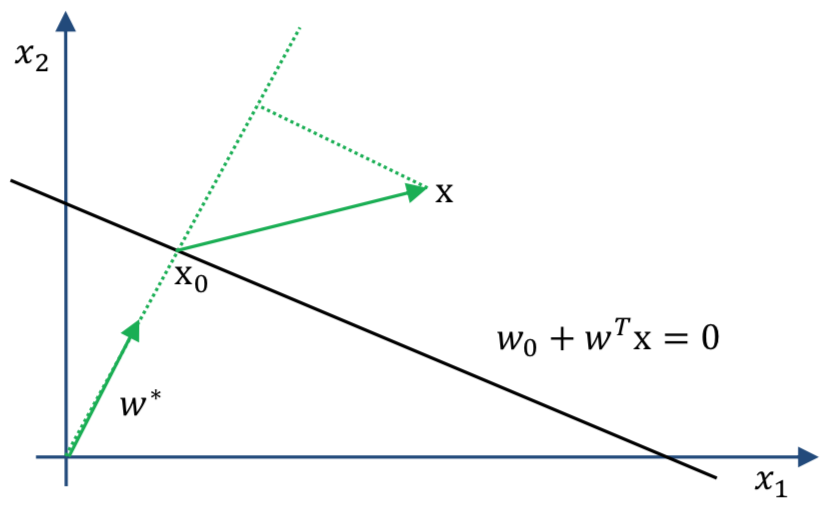
\includegraphics[width=6cm]{images/perceptron_decbound.png}
\end{wrapfigure} 

If you consider perceptron, is there any implicit cost in the perceptron rule? To understand this we need a little bit of math. \\
%Perceptron are more or less lines. 
Let's consider the hyperplane (affine set) $\boldsymbol{L \in \mathbb{R}^2}$ [the decision boundary of the perceptron]:
%(min 13:43 reg 3, slide 49)

\begin{center}
    $L: w_{0}+w^{T} x=0$
\end{center}
Let's think about our problem in a 2-dim space: the perceptron is deciding between a +1 or a -1. For any two points $\mathrm{x}_{1}$ and $\mathrm{x}_{1}$ on $\boldsymbol{L \in \mathbb{R}^2}$, it means that $w_0 + w^T \mathrm{x}_{1}=0$ and $w_0 + w^T \mathrm{x}_{2}=0$. We have that the \textit{normal vector} of $\mathrm{x}_{1} - \mathrm{x}_{2}$ (which specify the direction of the hyperplane $\boldsymbol{L}$) is $w^T$, in fact:
\begin{center}
    $w^{T}\left(\mathrm{x}_{1}-\mathrm{x}_{2}\right)=0$
\end{center}
%$\mathrm{x}_{1}$ is a point and you can think as a vector going from the origin to that point (slide 49), $\mathrm{x}_{2}$ is the other vector; so $\mathrm{x}_{1}-\mathrm{x}_{1}$ is the other vector (la differenza tra i due). 

The \textit{versor normal} to $\boldsymbol{L \in \mathbb{R}^2}$ is then: $ w^* = \frac{w}{||w||}$. For any point $x_0$ in $\boldsymbol{L \in \mathbb{R}^2}$ we have:
$$
w^{T} x_{0}+w_{0}=0 \rightarrow
w^T x_0 = -w_0
$$
$w$ is something like $(\mathrm{w}_{1},\mathrm{w}_{2})$ so it's a vector as well. \\
%When does the product between the two vectors become equal to zero? As always, when they are orthogonal, so you can interpret $w$ as an orthogonal vector to the decision boundary. If you want to normalize you can just divide by the norm, obtaining the versor $w^{*}=w /\|w\|$ which is the normal normal to my decision boundary. For any point $x_{0}$ on the line, being on the line means that $w^{T} x_{0}+w_{0}=0$, so $w^{T} x_{0}=-w_{0}$. 
%There is this nice property: you take the equation of the line you compute at any point in space and divide by the norm of the weights, this is the distance of this point from the line itself::
Taking any point $\boldsymbol{x}$ in $\mathbb{R}^2$ and considering the difference vector of $\boldsymbol{x} - \mathrm{x}_{0}$, the projection on the direction of $W^*$ of that vector is: 
$$
w^{*T} (\boldsymbol{x} - \mathrm{x}_{0}) = \frac{w^T}{||w||} (\boldsymbol{x} - \mathrm{x}_{0}) = \frac{1}{||w||} w^T(\boldsymbol{x} - \mathrm{x}_{0}) = \frac{1}{||w||} (w^T\boldsymbol{x} - w^{T}\mathrm{x}_{0}) = \frac{1}{||w||} (w^T\boldsymbol{x} + w_0)
$$
where $w^{*T} (\boldsymbol{x} - \mathrm{x}_{0})$ corresponds to the distance of x from the hyperplane $\boldsymbol{L}$ [the projection], so $(w^T\boldsymbol{x} + w_0)$ is proportional to the distance of $\boldsymbol{x}$ from the plane defined by $(w^T\mathrm{x} + w_0)=0$ [$\boldsymbol{L}$].\\
To sum up, the previous procedure means that the distance of a point $\boldsymbol{x}$ from the hyperplane (i.e. the projection of $(\boldsymbol{x} - \mathrm{x}_{0})$ on the direction of $w^*$, the normal versor of the hyperplane) is \textit{equal} to $(w^T\boldsymbol{x} + w_0)$ multiplied by a scalar factor $\frac{1}{||w||}$.\\
%Basically this term is proportional to the distance of $x$ from the plane defined by $\left(w^{T} x+w_{0}\right)=0$. 
If the vector is above the line, the distance is positive; if the vector is below the line then the distance is negative. \\

\textit{Perceptron Learning Algorithm} The output of the perceptron can be +1/-1:
\begin{itemize}
    \item If an output $t=+1$ is misclassified (your prediction is $t=-1$), then $\left(w^{T} x+w_{0}\right) < 0$
    \item On the other side if the output is $t=-1$ and your prediction is $t=+1$, then $\left(w^{T} x+w_{0}\right) > 0$
\end{itemize}{}

%that means that errors can be of two types:
%\begin{itemize}
%    \item +1 but $\left(w^{T} x+w_{0}\right)<0$;
%    \item -1 but $\left(w^{T} x+w_{0}\right)>0$.
%\end{itemize}

We can see that in errors the product of the two (classification label and $\left(w^{T} x+w_{0}\right)$) is always negative, so we can write this error which tries to minimize the product between the target and the distance of a misclassified point $x_i$ from the hyperplane:
%(which is the perceptron boundary, as we just shown):
\begin{center}
    $D\left(w, w_{0}\right)=-\sum_{i \in M} t_{i}\left(w^{T} x_{i}+w_{0}\right)$
\end{center}
%Basically if you have an error you want to minimize the product of $t_{i}$ and the distance; 
where $M$ is the set of misclassified points. \\

%To minimize this we could compute it for all errors and then simply doing stochastic gradient descend, this is the batch approach. On other option is just doing stochastic gradient descent on each single error, so it's the stochastic gradient descent of this error function. Gradient descent w.r.t. the model parameters is:
Minimizing by stochastic gradient descent the error function $d(w,w_0)$, the gradients with respect to the model parameters are:
\begin{center}
    $\frac{\partial D\left(w, w_{0}\right)}{\partial w}=-\sum_{i \in M} t_{i} \cdot x_{i} \quad \frac{\partial D\left(w, w_{0}\right)}{\partial w_{0}}=-\sum_{i \in M} t_{i}$
\end{center}
Stochastic gradient descent applies for each misclassified point:
\begin{center}
    $\left(\begin{array}{l}{w^{k+1}} \\ {w_{0}^{k+1}}\end{array}\right)=\left(\begin{array}{l}{w^{k}} \\ {w_{0}^{k}}\end{array}\right)+\eta\left(\begin{array}{c}{t_{i} \cdot x_{i}} \\ {t_{i}}\end{array}\right)$
\end{center}
This is exactly Hebbian Learning:
%, and this came after Hebbian Learning and they did not know that. This is the right thing to do: 
model the error as the distance of points wrongly classified from the boundary. This is different because it does not say anything about probabilities. The perceptron is a classical \textit{discriminative} approach, on the contrary feed forward neural network trained with cross-entropy is a classical \textit{generative} approach (generative methods try to predict some a-posteriori probability, discriminative approaches instead don't care at all of probabilities, they just take a line).

Anyways this latter thing is not used anymore because you need to do this update for each misclassified point and it could be very long.
%, but it's just to show that you can have several error functions and error functions describe a problem, and even the perceptron was performing in a way a minimization problem via backpropagation. 

These error functions are nowadays called \textbf{Loss Functions}. The term loss actually comes from stochastic risk minimization, where you want to minimize the risk and integrate the loss over all possible outcomes etc., but for us it's something that you want to minimize. How do I design error functions? You can use the knowledge about the data distribution or you can have some background information (cross-entropy and perceptron are built in different ways in this sense) or finally, you can use your creativity.